\chapter{Diskussion der Ergebnisse}\label{cha:Robustheit}
Dieses Kapitel dient der Diskussion des in Kapitel \ref{cha:Regler} entworfenen Verkopplungsreglers. Dabei wird insbesondere auf die Erfüllung der in Kapitel \ref{cha:Anforderungen} gestellten Anforderungen eingegangen. Der Entwurf wird zum einen am nominellen Modell, ohne Wirkung von Parameterschwankungen, evaluiert und zum anderen für ein Modell, welches von Parameterunsicherheiten in Form von Abweichungen in der Flugzeugmasse beeinflusst wird. Dabei wird sowohl das um den Arbeitspunkt linearisierte Modell als auch das nichtlineare Modell verwendet. Abschließend werden in diesem Kapitel anhand des nominellen Modells strukturelle Erweiterungen erläutert, die die Robustheit bezüglich von außen auf die Flugzeuge wirkenden Störgrößen begünstigen.

\section{Ergebnisse des linearisierten Modells ohne Stellgrößenbeschränkung}
Zunächst soll nur das nominelle Modell betrachtet werden. In Abbildung \ref{fig:pzmap_controlled} ist dazu die Lage der Pol- und Nullstellen des geregelten Systems mit dem vorgegebenen Polgebiet dargestellt. In Abbildung \ref{fig:pzmap_controlled_ohnezoom} ist gut zu erkennen, dass die invarianten Nullstellen des Systems durch entsprechende Platzierung von Eigenwerten kompensiert werden. Abbildung \ref{fig:pzmap_controlled_zoom} zeigt außerdem deutlich, dass alle Pole, wenn auch teilweise recht nah am Rand, innerhalb des vorgegebenen Polgebiets platziert werden.

\begin{figure}[h] % figure pzmap linear
	\centering
	\begin{subfigure}{.49\textwidth}
		\centering
		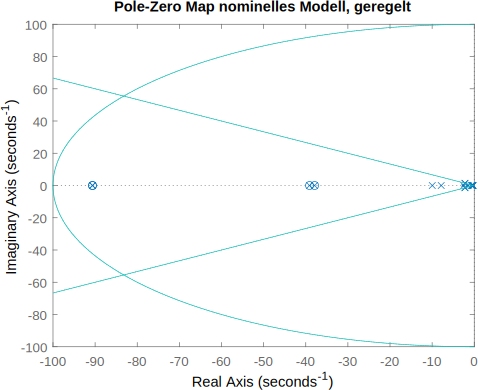
\includegraphics[width=\linewidth]{./Bilder/pzmap_controlled.eps}
		\caption{Vollständiges Polgebiet}
		\label{fig:pzmap_controlled_ohnezoom}
	\end{subfigure}
	\hfill
	\begin{subfigure}{.49\textwidth}
		\centering
		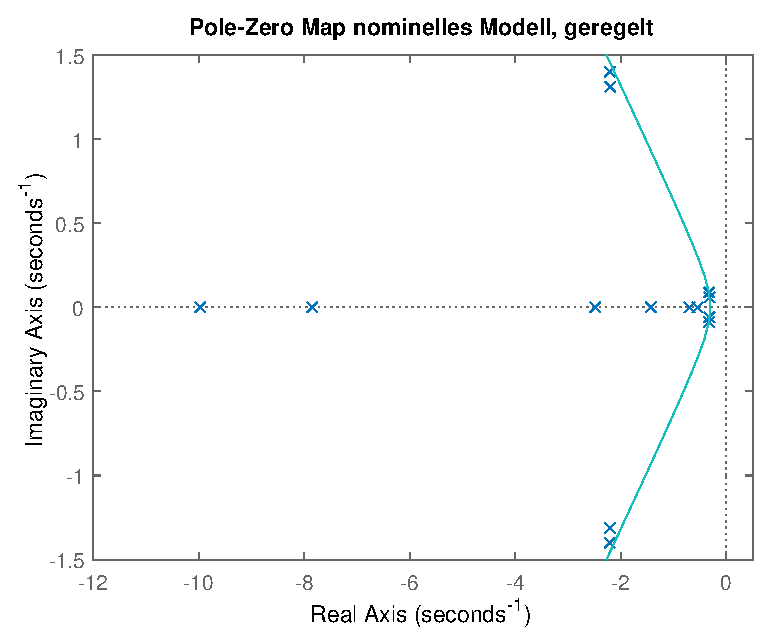
\includegraphics[width=\linewidth]{./Bilder/pzmap_controlled_zoom.eps}
		\caption{Polgebiet mit Fokus auf den Ursprung}
		\label{fig:pzmap_controlled_zoom}
	\end{subfigure}
	\caption{Pol-/ Nullstellendiagramm des geregelten linearen Systems}
	\label{fig:pzmap_controlled}
\end{figure}

In den Abbildungen \ref{fig:outputs_linear_ohne_stellbesch} und \ref{fig:stellgr_linear_ohne_stellbesch} sind die Sprungantworten sowie die Stellgrößenverläufe des linearen Modells ohne Einfluss der Stellgrößenbeschränkungen für Änderungen um den Arbeitspunkt dargestellt. 
\begin{figure}[H] % figure outputs nur linear ohne stellgrößenbeschränkung
	\centering
	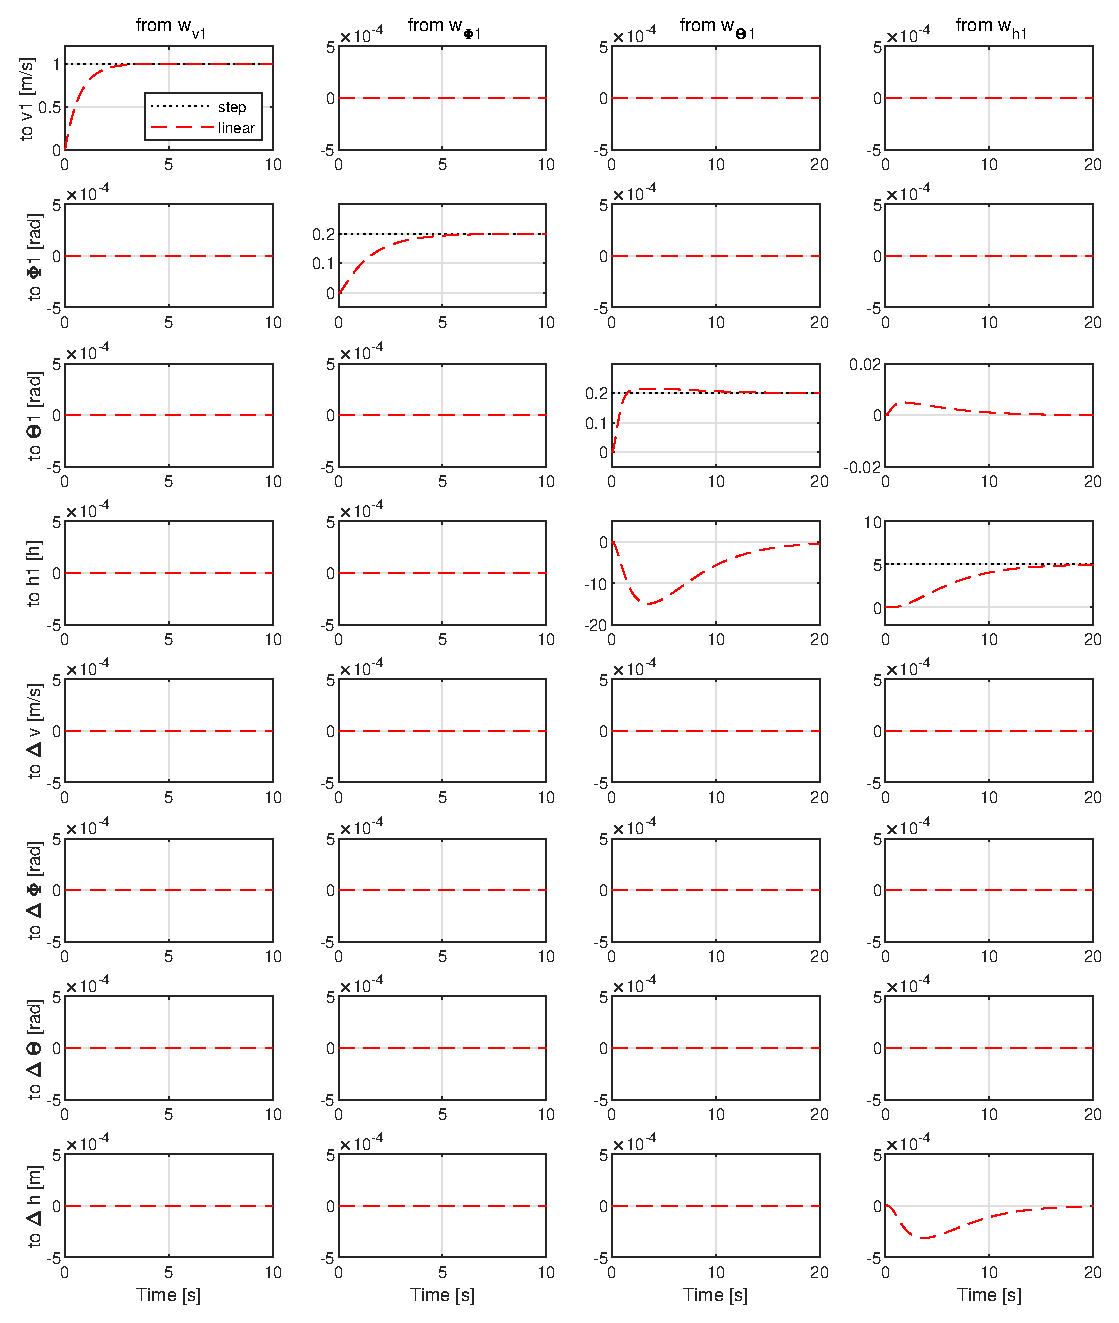
\includegraphics[width=\linewidth]{./Bilder/outputs_lin_ohne_beschr_um_AP.eps}
	\caption{Sprungantworten \textbf{ohne} Wirkung der Stellgrößenbeschränkung bei sprungförmigen Änderungen um den Arbeitspunkt, lineares System}
	\label{fig:outputs_linear_ohne_stellbesch}
\end{figure}
Für die Führungsgrößen $v_1$ und $h_1$ werden Sprünge von $\valunit{1}{m/s}$ respektive $\valunit{5}{m}$ ausgehend vom eigentlichen Arbeitspunkt vorgegeben. Für die beiden Eulerwinkel $\Phi_1$ und $\Theta_1$ werden Sprünge von jeweils $\valunit{0.2}{rad}$ gewählt, was $\valunit{11.46}{\degree}$ entspricht. Bei Betrachtung der Sprungantworten in Abbildung \ref{fig:outputs_linear_ohne_stellbesch} ist gut zu erkennen, dass die Verkopplung für alle Größen erfolgreich ist. Lediglich Führungssprünge auf $h_1$ führen dazu, dass $\Delta h$ minimal schwingt, was nach etwa \valunit{15}{s} allerdings wieder abgeklungen ist. Es ist außerdem zu erkennen, dass $v_1$ seinen Endwert nach \valunit{2}{s} ohne Überschwingen und entkoppelt von den anderen Ausgängen des ersten Flugzeugs stationär genau erreicht. Das gleiche gilt für $\Phi_1$ nach \valunit{5}{s}. Bei Betrachtung der Sprungantworten von $\Theta_1$ und $h_1$ fällt zudem auf, dass sich diese Größen gegenseitig beeinflussen, was durch die Wahl der Übertragungsmatrix zulässig ist. Die anderen Ausgangsgrößen von Flugzeug 1 werden dabei nicht beeinflusst. Diese beiden Größen benötigen jeweils etwa \valunit{15}{s} bis zum Erreichen des stationären Endwerts. Ein Sprung auf $\Theta_1$ führt dabei zu einem Höhenverlust von \valunit{15}{m} bevor die Höhe wieder auf ihren Sollwert zurückgestellt wird, während ein Höhensprung lediglich einen sehr geringen Einfluss auf $\Theta_1$ hat. 
\begin{figure}[H] % figure nur linear stellgrößen
	\centering
	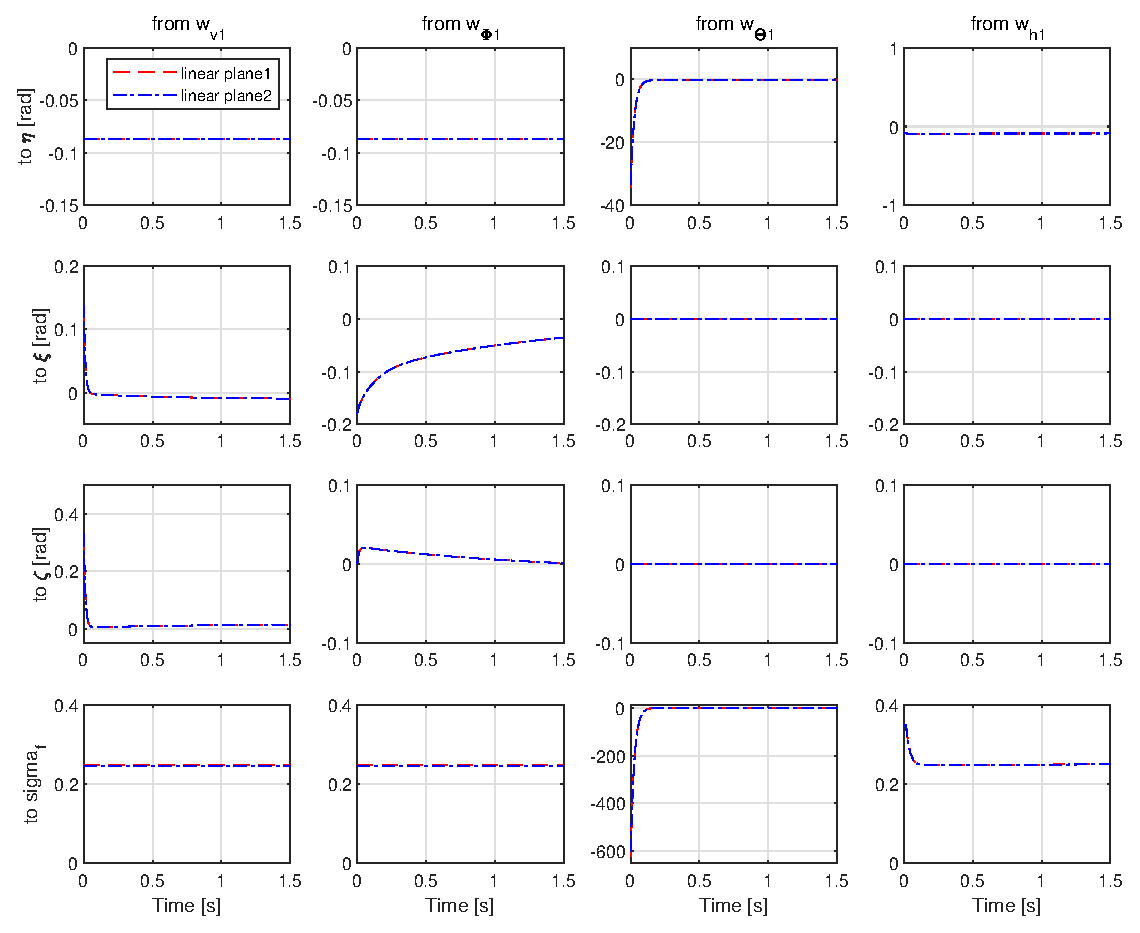
\includegraphics[width=\linewidth]{./Bilder/stellgr_linear_ohne_stellbeschr.eps}
	\caption{Stellgrößen \textbf{ohne} Wirkung der Stellgrößenbeschränkung bei sprungförmigen Änderungen um den Arbeitspunkt, lineares System}
	\label{fig:stellgr_linear_ohne_stellbesch}
\end{figure}
Bei Betrachtung der Stellgrößenverläufe in Abbildung \ref{fig:stellgr_linear_ohne_stellbesch} fällt zunächst auf, dass diese für die beiden Flugzeuge nahezu identisch sind. Zudem lässt sich feststellen, dass beim Aufschalten von Führungssprüngen - mit Ausnahme von $\Theta_1$ - die Stellgrößenbeschränkungen nicht verletzt werden. Bei $\Theta_1$ hingegen führt schon ein relativ geringer Sprung zu sehr hohen Stellgrößen, die jenseits der Grenzwerte für die Stellgrößen liegen. Bei Einführung der Stellgrößenbeschränkungen wird diese Eigenschaft zu unerwünschtem bis hin zu instabilem Systemverhalten führen. 

\section{Vergleich des linearen Modells mit dem nichtlinearen Modell unter Verwendung der Stellgrößenbeschränkungen}
Im Folgenden wird ebendieser Fall verdeutlicht. Die Abbildungen \ref{fig:stellgr_linear_nlinear_mit_stellbeschr} und \ref{fig:outputs_linear_nlinear_mit_stellbeschr} zeigen das Verhalten des linearen Modells im Vergleich mit dem nichtlinearen Modell unter Einfluss der Stellgrößenbeschränkung für sprungförmige Änderungen um den Arbeitspunkt. 
\begin{figure}[H] % figure stellgrößen linear und nlinear mit stellgrößenbeschränkung
	\centering
	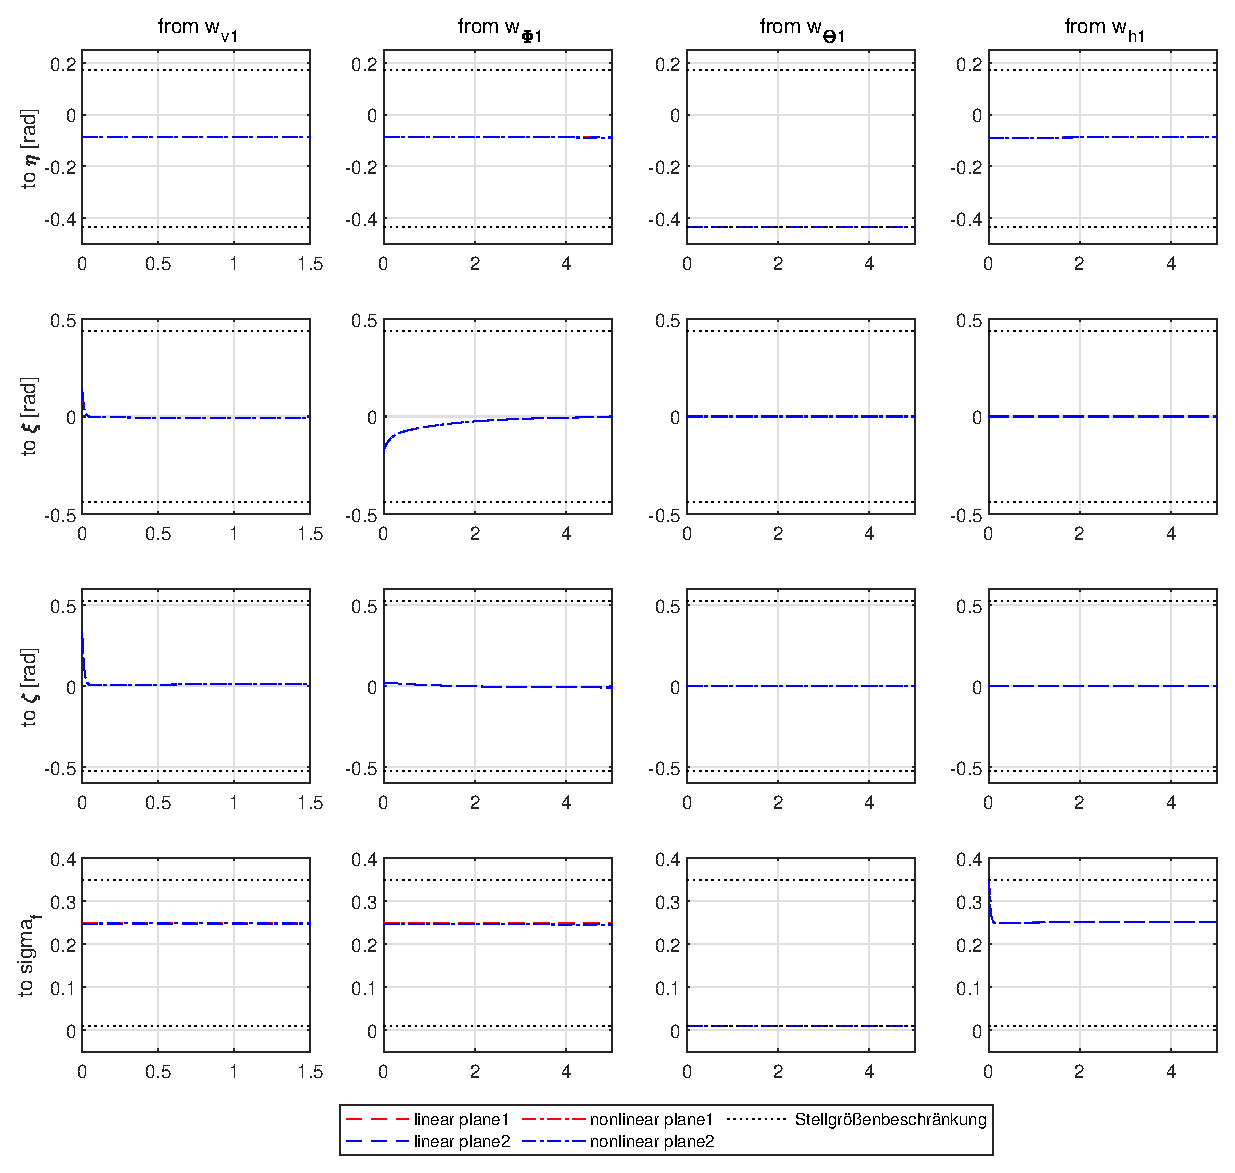
\includegraphics[scale=0.75]{./Bilder/stellgr_linear_nlinear_mit_stellbeschr_plot_stellgr.eps}
	\caption{Stellgrößen des linearen und nichtlinearen Modells \textbf{mit} Wirkung der Stellgrößenbeschränkung bei sprungförmigen Änderungen um den Arbeitspunkt}
	\label{fig:stellgr_linear_nlinear_mit_stellbeschr}
\end{figure}
Die gepunkteten Linien stellen die jeweiligen Stellgrößenbeschränkungen dar. Bei Betrachtung der dritten Spalte von Abbildung \ref{fig:stellgr_linear_nlinear_mit_stellbeschr} fällt zunächst auf, dass die Stellgrößen $\eta$ und $\tn{sigma}_f$ bei Anregung von $\Theta_1$ durch die unteren Grenzwerte der Stellgrößen begrenzt werden. Wie in Abbildung \ref{fig:outputs_linear_nlinear_mit_stellbeschr} zu erkennen ist, führt dies zu unerwünschtem Systemverhalten (Änderung von $\Phi_1$ um mehr als \valunit{110}{\degree}), was darauf zurückzuführen ist, dass die Stellgrößenbeschränkung in diesem Fall wie eine Öffnung der Regelschleife wirkt. Es kann auf Zustandsänderungen nicht mehr sinngemäß reagiert werden, wodurch sich das System schnell vom Arbeitspunkt entfernt. Das Modell verliert damit für diesen Bereich seine Gültigkeit. Dieser Einfluss wirkt sich beim linearen Modell allerdings stärker aus als beim nichtlinearen Modell. Dies zeigt sich darin, dass die Verkopplung beim nichtlinearen Modell, insbesondere bei der Höhe, besser erreicht wird.
\begin{figure}[H] % figure outputs linear und nlinear mit stellgrößenbeschränkung
	\centering
	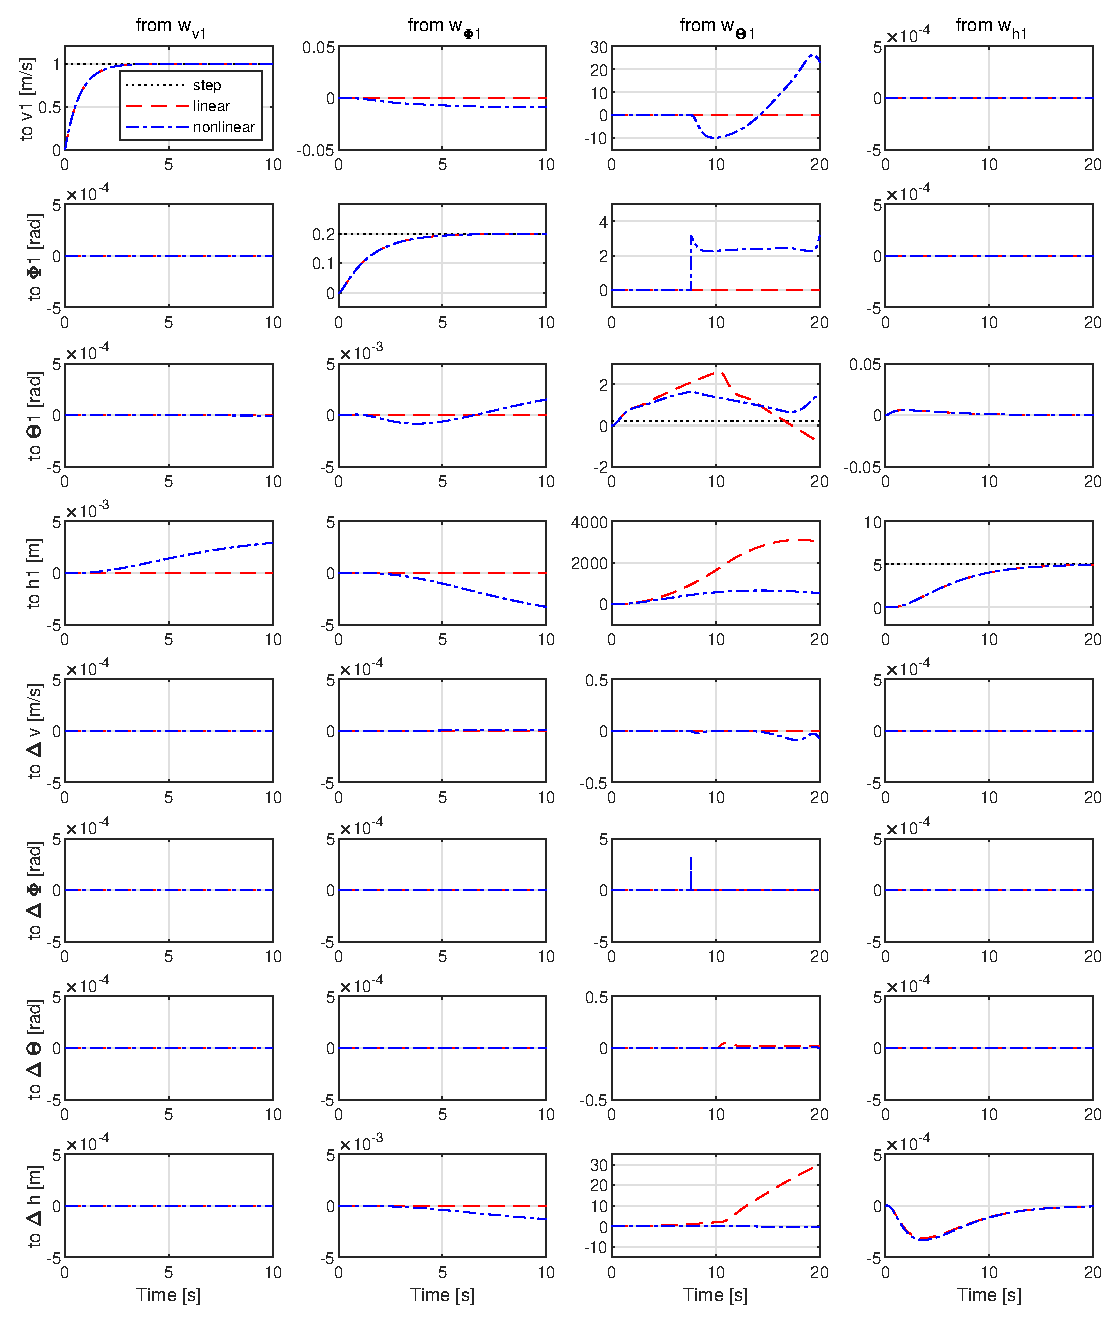
\includegraphics[width=\linewidth]{./Bilder/outputs_lin_nlin_mit_beschr_um_AP.eps}
	\caption{Sprungantworten des linearen und nichtlinearen Modells \textbf{mit} Wirkung der Stellgrößenbeschränkung bei sprungförmigen Änderungen um den Arbeitspunkt}
	\label{fig:outputs_linear_nlinear_mit_stellbeschr}
\end{figure}
Des Weiteren fällt auf, dass bei den Anregungen von $v_1, \Phi_1$ und $h_1$ die Verkopplung sowohl für das lineare als auch für das nichtlineare Modell erreicht wird. Außerdem lässt sich feststellen, dass die beiden Modelle am Arbeitspunkt zwar relativ gut miteinander übereinstimmen, es aber teilweise leichte Abweichungen gibt. Diese Unterschiede sind unter anderem in der Übertragungsfunktion $\Phi_1 \rightarrow h_1$ zu erkennen und führen dazu, dass die Entkopplung der einzelnen Ein- und Ausgänge von Flugzeug 1 beim nichtlinearen Modell teilweise nicht erreicht wird. Sie sind darauf zurückzuführen, dass das lineare Modell das Systemverhalten des nichtlinearen Modells bei Abweichungen vom Arbeitspunkt nicht mehr exakt widerspiegelt. Das lineare Modell ist nur genau im Arbeitspunkt exakt. Zudem zeigt Abbildung \ref{fig:stellgr_linear_nlinear_mit_stellbeschr}, dass bei den entsprechenden Sprunghöhen für $v_1, \Phi_1$ und $h_1$ die Stellgrößenbeschränkungen weder beim linearen noch beim nichtlinearen Modell verletzt werden. 

\subsection{Verkopplung der Flugzeugpositionen}
Eine weitere Anforderung an die Regelung ist die Verkopplung der Flugzeugpositionen. Diese wird im Folgenden betrachtet und analysiert. Der Abstand der Flugzeuge bezüglich des erdfesten Referenzkoordinatensystems ist in Abbildung \ref{fig:distance_xyz_nlinear} für das nichtlineare Modell dargestellt. Es ist gut zu erkennen, dass bei allen Sprunganregungen mit Ausnahme von $\Theta_1$ die Verkopplung der Flugzeugpositionen über den Simulationszeitraum gegeben ist. Der Abstand in Richtung der $y-$Achse beträgt null Meter. Für die $x-$Achse und die $z-$Achse beträgt der Abstand jeweils \valunit{10}{m}, was den gewünschten Werten im Arbeitspunkt entspricht. Die Darstellung über den relativ kurzen Zeitraum soll jedoch keine Einschränkung sein, da die Zustände nach Ablauf der Simulation bereits im eingeschwungenen Zustand sind. Das heißt, auch über einen längeren Zeitraum oder bei mehrfacher Anregung wäre die Verkopplung gewährleistet. Eine Anregung von $\Theta_1$ führt allerdings zu einer Abweichung der Werte von ihren Sollwerten und damit zu einem Verlust der Verkopplung der Positionen. 
\begin{figure}[h] % figure distanz zwischen flugzeugen
	\centering
	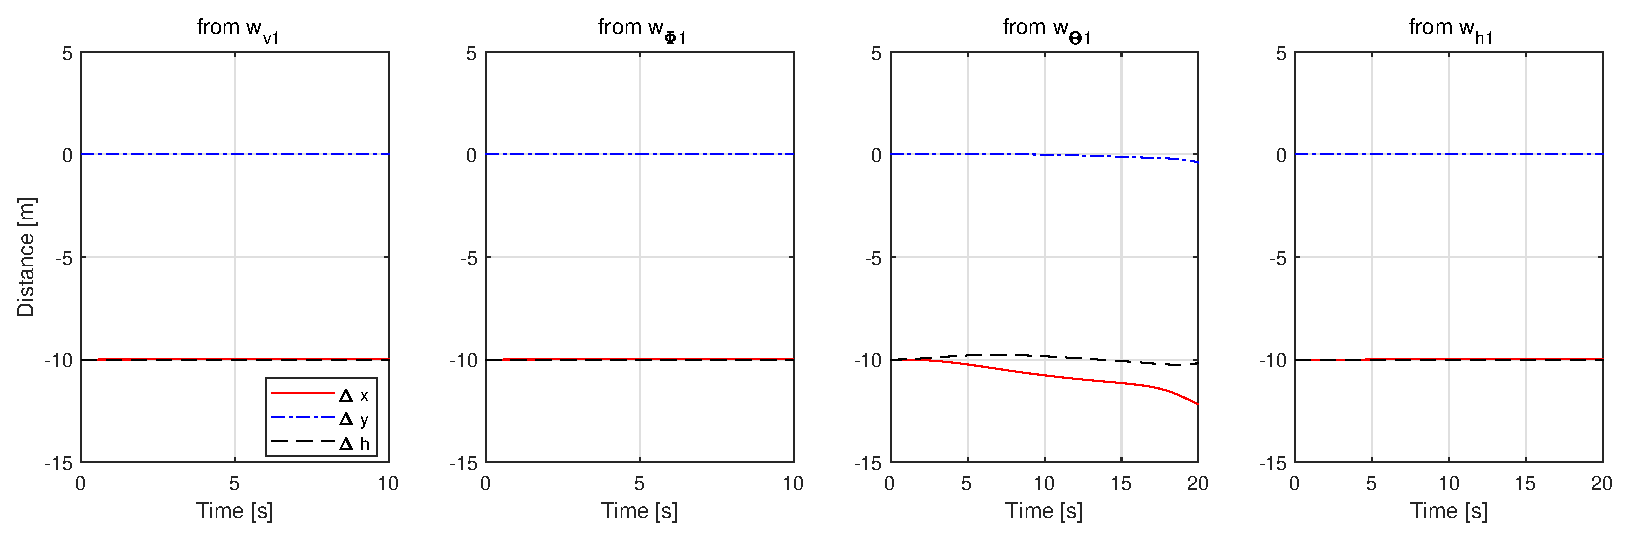
\includegraphics[scale=0.6]{./Bilder/distance_xyz_nlinear.eps}
	\caption{Abstand der Flugzeuge bezüglich des erdfesten Referenzsystems für das nichtlinearen Modell}
	\label{fig:distance_xyz_nlinear}
\end{figure}
Als Zwischenfazit lässt sich also festhalten, dass die Regelung prinzipiell dazu in der Lage ist, die Flugzeuge miteinander zu verkoppeln und auch die Entkopplung der Führungsgrößen von Flugzeug 1 wie gewünscht erreicht wird. Führungssprünge des Nickwinkels führen allerdings zu enorm hohen Stellgrößen, welche durch die Stellgrößenbeschränkung begrenzt werden und dadurch zum Verlust der gewünschten Eigenschaften führen. Die Regelung reagiert sehr sensitiv auf derartige Änderungen.

\section{Ergebnisse Parameterschwankungen der Flugzeugmasse}\label{sec:Parameterschwankungen}
Nachdem nun das Systemverhalten des linearen und des nichtlinearen Modells für das nominelle Modell miteinander verglichen und hinsichtlich der Anforderungen an die Regelung diskutiert wurde, soll nun der Einfluss von Parameterschwankungen in Form von unterschiedlichen Flugzeugmassen am nichtlinearen Modell analysiert werden. 
\subsection{Einführung der Modelle unter Parameterschwankung}
Die Parameterschwankung wirkt dabei so, dass zu Beginn der Betankung Flugzeug 1 (Tankflugzeug) zusätzliche zu seiner eigenen Masse die Masse des Treibstoffs transportiert, während Flugzeug 2 (betanktes Flugzeug) nur seine eigene Masse transportiert (siehe Kapitel \ref{cha:ZweiFlieger}). Es gilt also 
\begin{align}
	m_1 = m + \sigma m_\tn{ks}, \qquad m_2 = m, \qquad \tn{mit} \, \sigma\in\lbrack0,1\rbrack,
\label{eq:massmodel1}
\end{align}
wobei die Parameterschwankung über den Parameter $\sigma$ zwischen 0 und \valunit{100}{\%} der gesamten Treibstoffmasse variiert werden kann. Dieser Fall wird nachfolgend als Modell 2 bezeichnet.
Nach Abschluss der Betankung hat das Tankflugzeug die Treibstoffmasse an das zu betankende Flugzeug abgegeben und es gilt entsprechend
\begin{align}
	m_1 = m , \qquad m_2 = m + \sigma m_\tn{ks}, \qquad \tn{mit} \, \sigma\in\lbrack0,1\rbrack.
\label{eq:massmodel2}
\end{align}
Dieser Fall wird nachfolgend als Modell 3 bezeichnet.

\subsection{Reglerauslegung mittels Multi-Modell-Ansatz}
Um einen bezüglich der Massenschwankung möglichst robusten Regler entwerfen, wird mit \texttt{gammasyn} versucht ein Regler mittels Multi-Modell-Ansatz auszulegen (siehe Kapitel \ref{cha:GrundlagenReg}). Dazu wird die Parameterschwankung zunächst sehr gering gewählt, damit die betrachteten Modelle nicht zu stark vom nominellen Modell abweichen. Die Treibstoffmasse wird mit $\sigma=0.1$ zu \valunit{1400}{kg} gewählt. Damit beträgt die Abweichung bezogen auf das nominelle Gewicht \valunit{1.167}{\%}. Es konnte festgestellt werden, dass unter Verwendung des in Kapitel \ref{cha:Regler} erklärten Polgebiets zur Einhaltung der Mindestanforderngen keine Lösung für das Optimierungsproblem gefunden werden kann. Daher werden die Anforderungen bezüglich des Polgebiets auf das Mindeste, die Forderung nach Stabilität, beschränkt und es wird als zulässiges Polgebiet der gesamte Bereich links der Imaginärachse gewählt. 

Abbildung \ref{fig:pzmap_multi_modell_ansatz} zeigt die Lage der Pol- und Nullstellen für die drei Modelle. Wie gut zu erkennen ist, können für keines der beiden Polgebiete alle Eigenwerte innerhalb des Polgebiets platziert werden. Es ist selbst bei der geringen Schwankung der Masse nicht möglich alle Eigenwerte links der Imaginärachse zu platzieren, was zu instabilem Verhalten führt. Es lässt sich schlussfolgern, dass kein robuster Verkopplungsregler für Schwankungen der Masse ausgelegt werden kann, der alle Systeme zumindest stabilisiert. 
\begin{figure}[h] % figure pzmap multimodell ansatz
	\centering
	\begin{subfigure}{.49\textwidth}
		\centering
		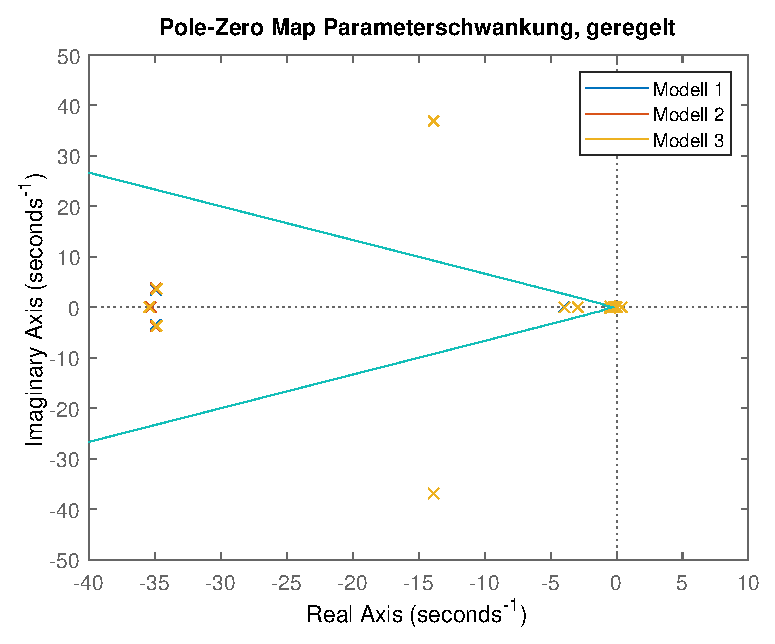
\includegraphics[width=\linewidth]{./Bilder/pzmap_multi_modell_10prozent_hyperbola.eps}
		\caption{Multi-Modell-Ansatz für das Polgebiet aus Kapitel \ref{cha:Regler}}
		\label{fig:pzmap_multi_modell_10prozent_hyperbola}
	\end{subfigure}
	\hfill
	\begin{subfigure}{.49\textwidth}
		\centering
		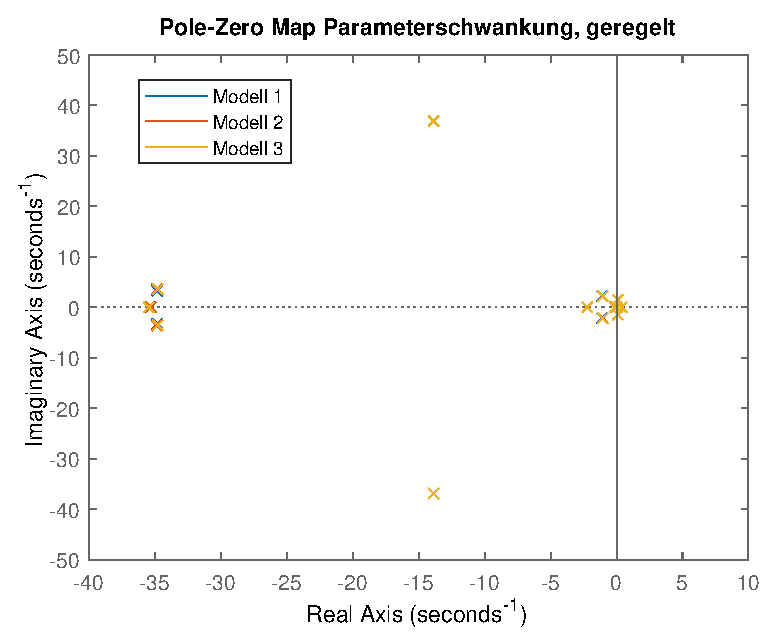
\includegraphics[width=\linewidth]{./Bilder/pzmap_multi_modell_10prozent_imag.eps}
		\caption{Multi-Modell-Ansatz für das Polgebiet links der Imaginärachse}
		\label{fig:pzmap_multi_modell_10prozent_imag}
	\end{subfigure}
	\caption{Pol-/ Nullstellendiagramm der drei Systeme unter Einfluss von Parameterschwankungen für das nominelle System (Modell 1), das System vor dem Betankungsvorgang (Modell 2) und das System nach Abschluss der Betankung (Modell 3) jeweils mit $\sigma=0.1$. Für jedes Polgebiet wird ein Regler mittels Multi-Modell-Ansatz ausgelegt.}
	\label{fig:pzmap_multi_modell_ansatz}
\end{figure}

\subsection{Reglerperformance von $\mat{K}_\tn{koppel}$ bezüglich der Modelle 2 und 3}
Nachdem zuvor gezeigt wurde, dass das System höchst sensitiv auf Schwankungen der Flugzeugmasse reagiert und mittels Multi-Modell-Ansatz nicht einmal Stabilität für alle drei Modelle gewährleistet werden kann, soll nachfolgend die Performance des in Kapitel \ref{cha:Regler} ausgelegten Verkopplungsreglers $\mat{K}_\tn{koppel}$ für die Modelle 2 und 3 evaluiert werden. Durch die unterschiedlichen Massen ergeben sich leicht abweichende Arbeitspunkte und dadurch auch unterschiedliche Systemmatrizen. Bei Vorgabe der entsprechenden Größen zur Bestimmung des Arbeitspunktes für den Geradeausflug (siehe Kapitel \ref{cha:Linearisierung}) ändern sich durch die zusätzliche Masse die Größen $w, \Theta, \eta$ und $\tn{sigma}_f$. Bei voller Treibstoffmasse ($\sigma=1$) gilt im Arbeitspunkt
\begin{align*}
w_\tn{AP1} = \valunit{-9.3012}{m/s}, \quad \Theta_\tn{AP1} = \valunit{-0.0619}{rad}, \quad \eta_\tn{AP1} = \valunit{-0.0954}{rad}, \quad \tn{sigma}_{f\tn{AP1}} = 0.2254
\end{align*}
für das auf \valunit{5000}{m} fliegende Flugzeug 1 und 
\begin{align*}
w_\tn{AP2} = \valunit{-9.2834}{m/s}, \quad \Theta_\tn{AP2} = \valunit{-0.0618}{rad}, \quad \eta_\tn{AP2} = \valunit{-0.0955}{rad}, \quad \tn{sigma}_{f\tn{AP2}} = 0.2252
\end{align*}
für das auf \valunit{5010}{m} fliegende Flugzeug 2. Abbildung \ref{fig:pzmap_controlled_schwankung} zeigt das Pol-/ Nullstellendiagramm für das nominelle Modell, Modell 2 und Modell 3. Wie aus der Abbildung zu erkennen ist, können bei der Regelung mit $\mat{K}_\tn{koppel}$ auch für die Modelle 2 und 3 die invarianten Nullstellen durch Eigenwerte kompensiert und alle Eigenwerte innerhalb des vorgegebenen Polgebiets platziert werden.
\begin{figure}[h] % figure pzmap multimodell
	\centering
	\begin{subfigure}{.49\textwidth}
		\centering
		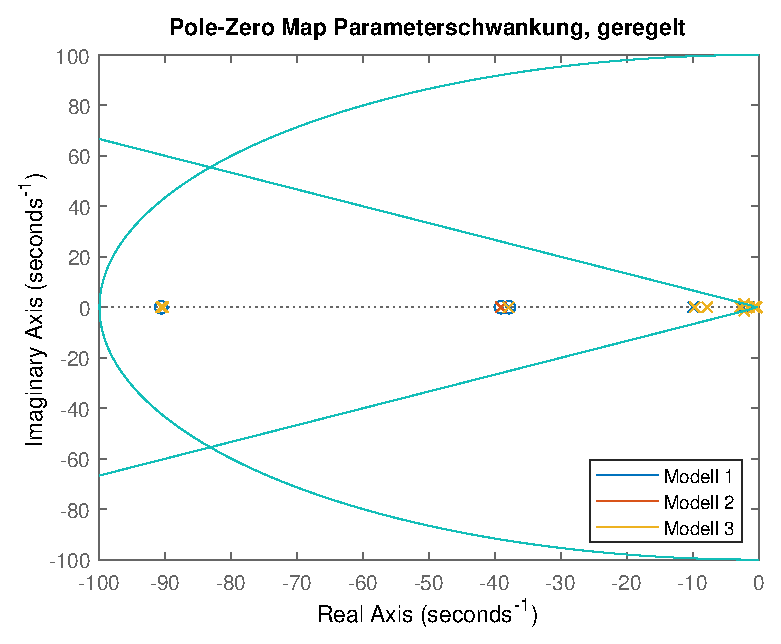
\includegraphics[width=\linewidth]{./Bilder/pzmap_controlled_schwankung.eps}
		\caption{Vollständiges Polgebiet}
		\label{fig:pzmap_controlled_schwankung_ohne_zoom}
	\end{subfigure}
	\hfill
	\begin{subfigure}{.49\textwidth}
		\centering
		\includegraphics[width=\linewidth]{./Bilder/pzmap_controlled_schwankung_zoom.eps}
		\caption{Polgebiet mit Fokus auf den Ursprung}
		\label{fig:pzmap_controlled_schwankung_zoom}
	\end{subfigure}
	\caption{Pol-/ Nullstellendiagramm der drei durch $\mat{K}_\tn{koppel}$ geregelten Modelle mit $\sigma=1$ (volle Tankladung).}
	\label{fig:pzmap_controlled_schwankung}
\end{figure}

Die Sprungantworten zu den Modellen 2 und 3 sowohl für den linearen als auch den nichtlinearen Fall sind in Abbildung \ref{fig:outputs_linear_nlinear_two_masses} dargestellt.
Wie bereits beim nominellen Modell, führen auch bei den Modellen 2 und 3 Führungssprünge auf $\Theta_1$ zu instabilem Verhalten. Da die starke Sensitivität des Systems bezüglich Änderungen von $\Theta_1$ bereits umfassend erläutert wurde, soll an dieser Stelle nicht weiter darauf eingegangen werden. Stationäre Genauigkeit ist bei Sprüngen auf $v_1$ und $\Phi_1$ bezüglich der jeweiligen Führungsgrößen nach wie vor gewährleistet. Es fällt allerdings auf, dass die Parameterschwankung der Masse Einfluss auf das Gesamtverhalten hat. So ist der Einfluss von $\Phi_1$ auf $v_1$ nun etwas stärker. Während die zusätzliche Masse beim linearen Modell keinen Einfluss auf die Höhe hat und sowohl die Sollhöhe $h_1$ gehalten wird als auch die Verkopplung der Höhe uneingeschränkt funktioniert, gilt dies für das nichtlineare Modell nicht. Es lässt sich erkennen, dass bei Sprüngen auf $v_1$ und $\Phi_1$ die Sollhöhe beim nichtlinearen Modell nicht gehalten werden kann und die zusätzliche Masse zu einem stationären Höhenverlust führt. Dadurch ist auch die Verkopplung der Höhen nicht mehr gewährleistet. Im Fall, dass Flugzeug 1 das schwerere Flugzeug ist (Modell 2), verliert es an Höhe, ohne dass Flugzeug 2 folgt, sodass der Abstand zwischen den beiden Flugzeugen größer wird. Im Fall, dass Flugzeug 2 bereits betankt wurde (Modell 3), ist es genau umgekehrt - die Flugzeuge nähern sich einander an. Dies gilt sowohl für Führungsgrößensprünge auf $v_1$ als auch auf $\Phi_1$. Außerdem entsteht im nichtlinearen Modell bei Sprüngen auf $v_1$ eine bleibende Abweichung für $\Delta v$ sowie $\Delta \Phi$. 

Führungssprünge bezüglich der Höhe haben keinerlei Einfluss auf $v_1$ und $\Phi_1$ und auch $\Theta_1$ wird nur leicht um den Arbeitspunkt herum ausgelenkt. Allerdings führt die Treibstoffmasse dazu, dass die stationäre Genauigkeit bezüglich der Höhe im nichtlinearen Modell verloren geht, sofern Flugzeug 1 das schwerere ist, da der Regler nicht dazu in der Lage ist diese Schwankung auszuregeln. Dies schlägt sich ebenfalls im verkoppelten Ausgang $\Delta h $ nieder. Ist Flugzeug 2 das schwerere, so wird der Sollwert bezüglich $h_1$ zwar stationär genau erreicht, jedoch gelingt es nicht, das schwerere Flugzeug 2 nachzuführen, sodass auch in diesem Fall eine bleibende Höhendifferenz entsteht. 
\begin{figure}[H] % figure sprungantworten zwei massenmodelle
	\centering
	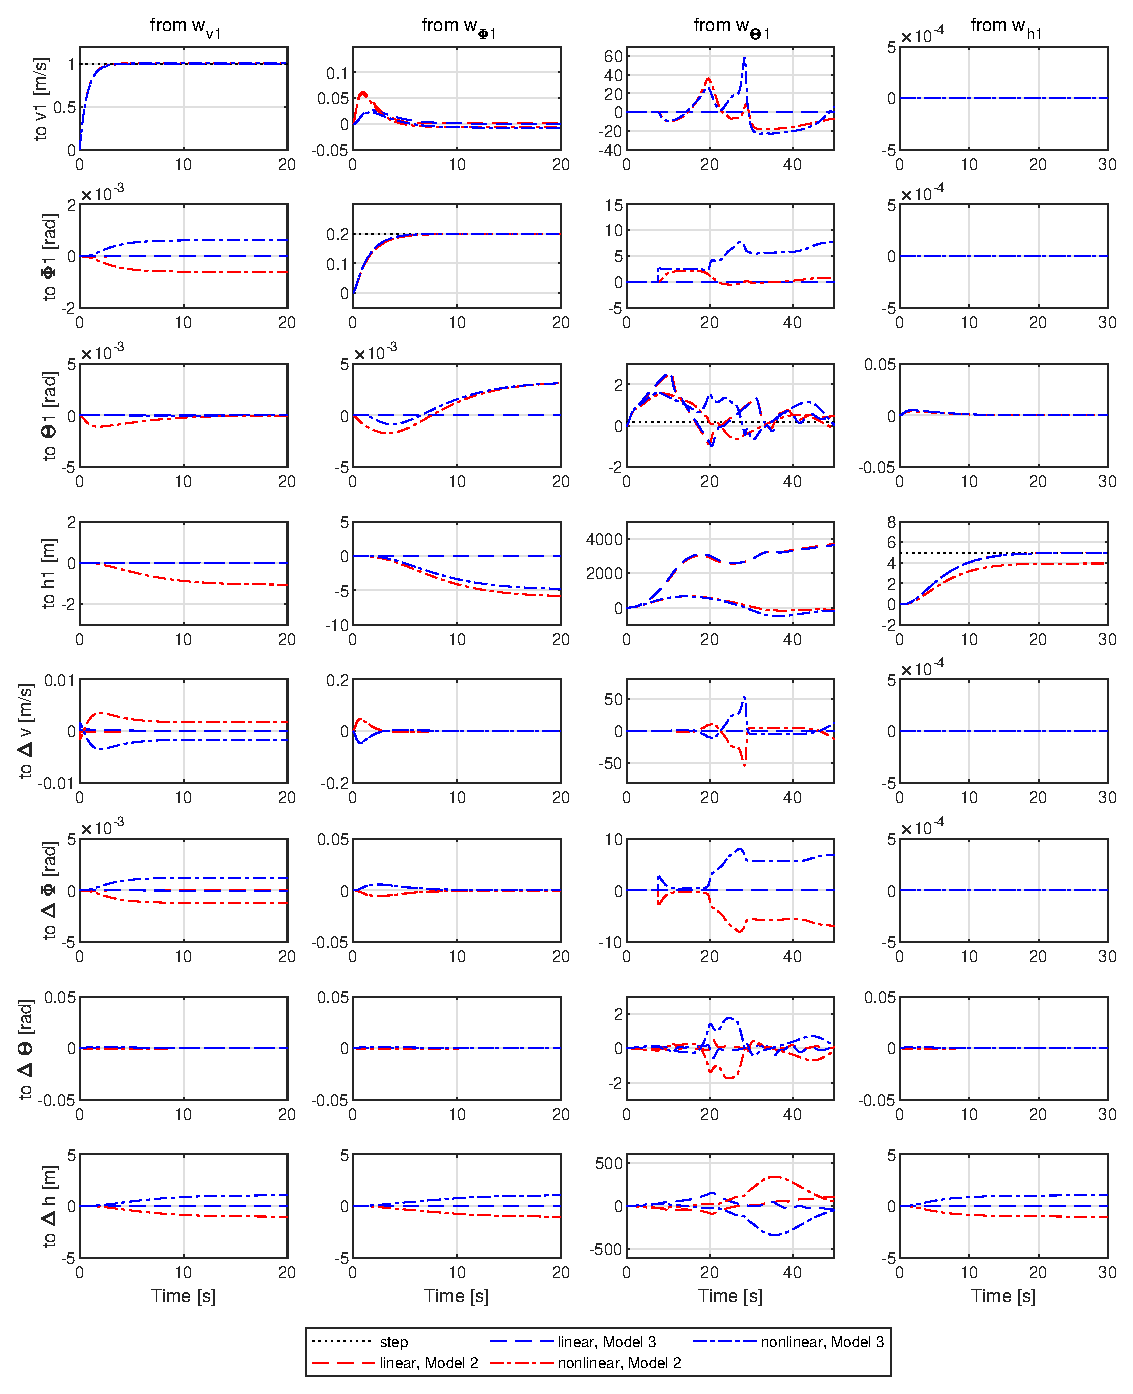
\includegraphics[width=\linewidth]{./Bilder/outputs_lin_nlin_two_masses_um_AP.eps}
	\caption{Sprungantworten der mit $\mat{K}_\tn{koppel}$ geregelten Modelle 2 und 3 für das lineare und nichtlineare Modell bei sprungförmigen Änderungen um den Arbeitspunkt}
	\label{fig:outputs_linear_nlinear_two_masses}
\end{figure}
Abbildung \ref{fig:distance_xyz_nlinear_twomassmodels} zeigt die Positionsdifferenz der beiden Flugzeuge für die Modelle 2 und 3. Es ist deutlich zu erkennen, dass die Regelung bei keinem der Modelle dazu in der Lage ist, die Positionen miteinander zu verkoppeln. Dies liegt daran, dass die Parameterschwankung zu einer Abweichung des Modells vom nominellen Modell führt, für das die Regelung ausgelegt wurde. Da die Positionen nicht Bestandteil der in der Zustandsrückführung geregelten Zustände sind, hat die Regelung keine Möglichkeit auf Positionsdifferenzen zu reagieren. Abweichungen in der Geschwindigkeit und den Kurswinkeln $\gamma$ und $\chi$ werden aufintegriert, ohne darauf Einfluss nehmen zu können. 
\begin{figure}[H] % figure positionsdifferenz zwei massenmodelle
	\centering
	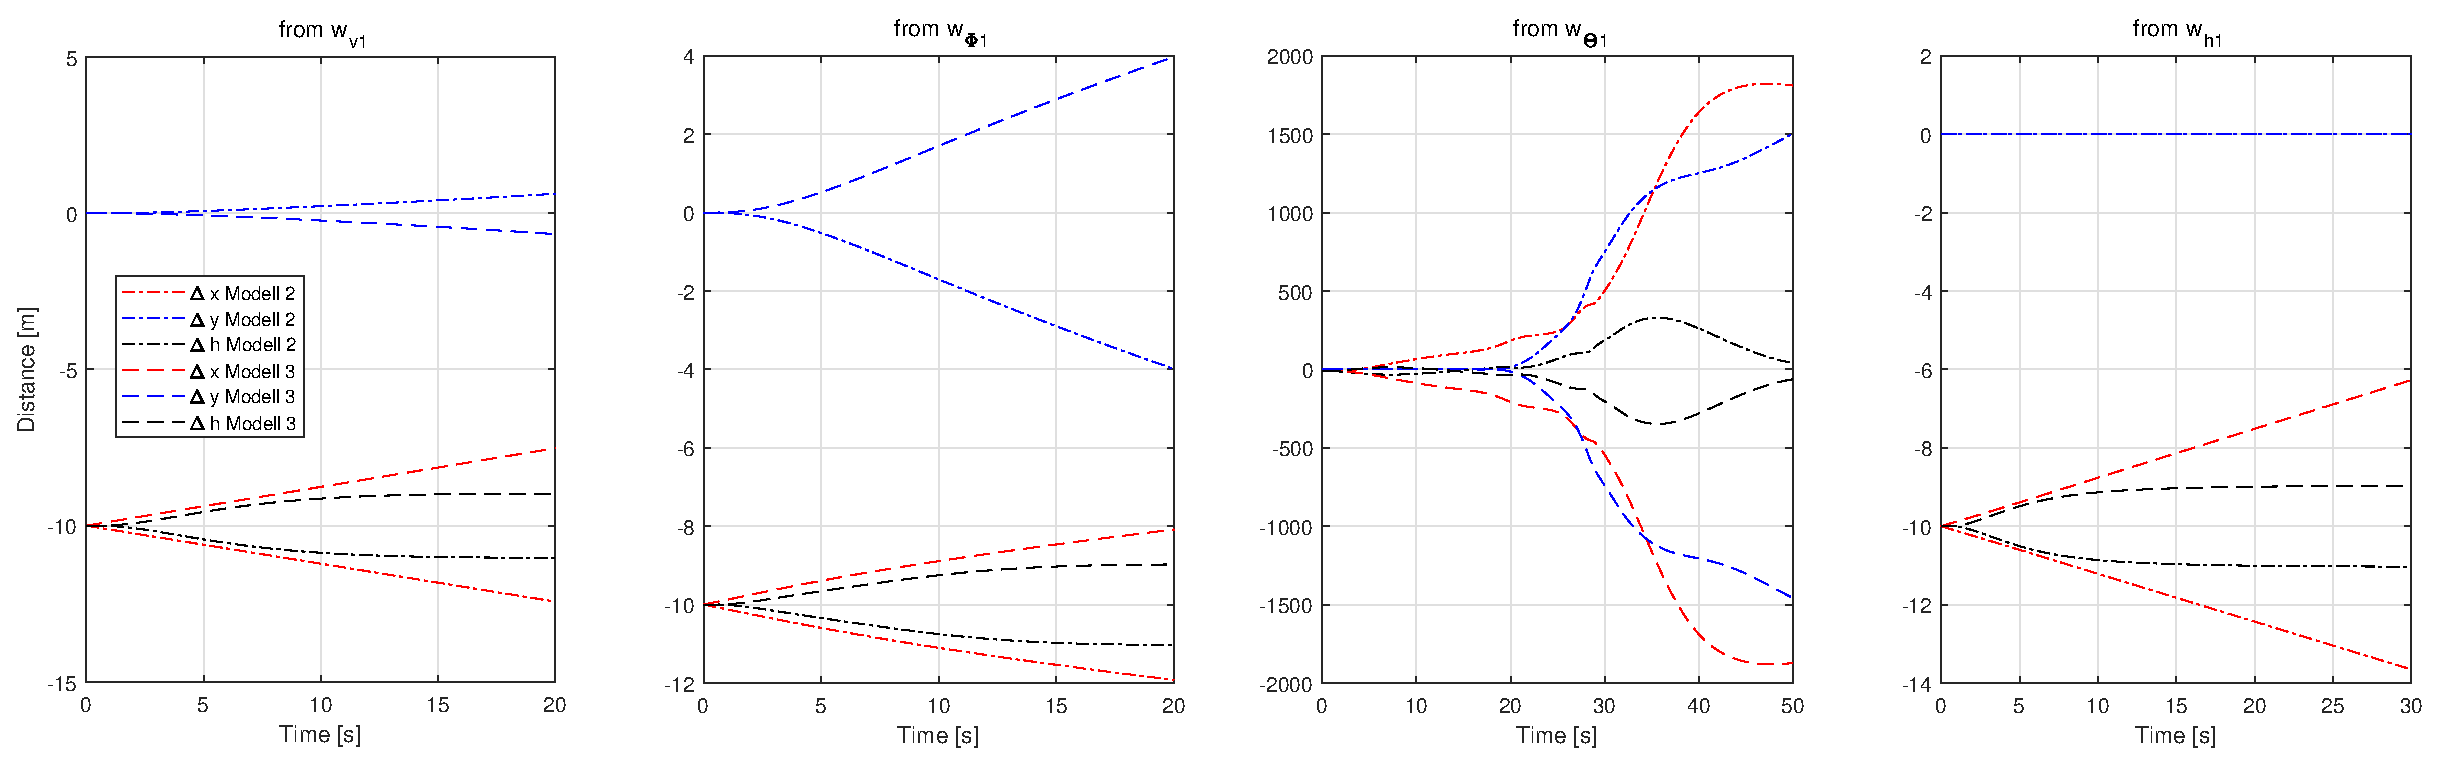
\includegraphics[width=\linewidth]{./Bilder/distance_xyz_nlinear_twomassmodels.eps}
	\caption{Abstand der Flugzeuge für die durch die durch die Massenschwankung beeinflussten nichtlinearen Modelle 2 und 3, geregelt mit $\mat{K}_\tn{koppel}$}
	\label{fig:distance_xyz_nlinear_twomassmodels}
\end{figure}
Damit lässt sich als Abschluss dieses Abschnitts festhalten, dass die Verkopplungsregelung den Einfluss der Parameterschwankung in der Flugzeugmasse nicht ausregeln kann. Bei Abweichung vom für die Reglerauslegung gültigen Modell, ist die Verkopplung der Flugzeuge nicht mehr gewährleistet. Geringere Schwankungen in der Masse führen zwar dazu, dass sich das System langsamer vom Arbeitspunkt entfernt und der Verlust der Verkopplung langsamer geschieht, das prinzipielle Systemverhalten ist allerdings gleich. Die Robustheit gegenüber derartigen Schwankungen ist nicht gegeben. 

\section{Strukturelle Erweiterung für das nominelles Modell}
Neben Parameterschwankungen können auch andere Störfaktoren das Systemverhalten beeinflussen. Äußere Störeinflüsse, die zum Beispiel in Form von Wind oder Luftlöchern in das System eingreifen, können dazu beitragen, dass das Systemverhalten instabil wird. Daher sollten diese durch die Regelung ausgeregelt werden. Die Störungen werden als sprungförmige Störgrößen, die auf die Zustände wirken, modelliert. Um derartige Störungen stationär genau ausregeln zu können, muss der Regelkreis vor dem Einfluss der Störgröße einen I-Anteil besitzen. Da dies durch den Verkopplungsregler nicht gewährleistet ist, wird im Folgenden zusätzlich zum Zustandsregler eine Ausgangsrückführung für die Führungsgrößen von Flugzeug 1 ausgelegt, die diese stationäre Genauigkeit bezüglich der Störungen sicherstellen soll. Die Regler werden anhand des nominellen Modells entworfen, da nur für dieses die Verkopplung erreicht wurde, und für das nichtlineare Modell evaluiert. Abbildung \ref{fig:blockschaltbild_unterlagerung} zeigt das Blockschaltbild der erweiterten Regelung.
 
\subsection{Entwurf der unterlagerten Regelung}
Für jeden der vier Führungsübertragungspfade 
\begin{align*}
	v_1 \rightarrow v_1, \qquad \Phi_1 \rightarrow \Phi_1, \qquad \Theta_1 \rightarrow \Theta_1, \qquad h_1 \rightarrow h_1 
\end{align*}
wird ein Regler mit einem I-Anteil so entworfen, dass vorhandene Null- und Polstellen, falls diese stabil sind, durch Hinzufügen zusätzlicher Null- und Polstellen, kompensiert werden. Der I-Anteil sorgt dafür, dass die Windstörungen stationär genau ausgeregelt werden können. Die Verstärkungsfaktoren der einzelnen Regler werden so gewählt, dass die hinzugefügten Polstellen möglichst den ursprünglichen entsprechen, sodass die Dynamik des äußeren Regelkreises der des inneren Regelkreises entspricht. Dabei wird die Annahme getroffen, dass die einzelnen Ausgänge nur von den jeweiligen Führungseingängen beeinflusst werden und die internen Verkopplungen von Flugzeug 1 so gering sind, dass sie keinen signifikanten Einfluss haben. Wie Abbildung \ref{fig:outputs_linear_nlinear_mit_stellbeschr} bereits gezeigt hat, ist diese Annahme mit Ausnahme von $\Theta_1$, welches bereits für kleine Anregungen aufgrund der Stellgrößenbeschränkung zu instabilem Verhalten führt, erfüllt.
\tikzstyle{block} = [draw, rectangle, 
minimum height=3em, minimum width=4em]
\tikzstyle{sum} = [draw, circle, node distance=1cm]
\tikzstyle{input} = [coordinate]
\tikzstyle{output} = [coordinate]
\tikzstyle{pinstyle} = [pin edge={to-,thin,black}]

\begin{figure}[h]
\centering
\begin{tikzpicture}[auto, node distance=3cm,>=latex']
% We start by placing the blocks
\node [input, name=input] {};
\node [sum, right of=input] (sum1) {};
\node [block, right of=sum1] (pidt_regler) {PIDT-Regler};
\node [block, right of=pidt_regler, pin={[pinstyle]above:Störung},
node distance=4cm] (system) {Verkoppeltes System};
\node [output, right of=system] (output) {};


% Once the nodes are placed, connecting them is easy. 
\draw [draw,->] (input) -- node {$\underline{w_1}$} (sum1);
\draw [->] (sum1) -- node {$\underline{e_1}$} (pidt_regler);
\draw [->] (pidt_regler) -- node {$\Delta\underline{w}_1$} (system);
\draw [->] (system) -- node [name=y] {$\underline{y}_1$}(output);
\draw [->] (y.south)  -- ++(0,-1.5cm) -| node[pos=0.99, right] {$-$} (sum1);
\end{tikzpicture}
\caption{Strukturbild der unterlagerten Regelung für das verkoppelte System.}
\label{fig:blockschaltbild_unterlagerung}
\end{figure}

Die vier Übertragungsfunktionen des inneren Regelkreises, der durch den Verkopplungsregler geregelt wird, lauten:
\begin{align}
G(s)_{v_1 \rightarrow v_1} &= \frac{1.4266}{s + 1.4266} \nonumber\\
G(s)_{\Phi_1 \rightarrow \Phi_1} &= \frac{5.4658}{(s+7.847)(s+0.6966)} \nonumber \\
G(s)_{\Theta_1 \rightarrow \Theta_1} &= \frac{6.82(s+0.492)(s+0.2129)}{(s^2+0.6348s+0.1042)(s^2+4.425s+6.854)} \\
G(s)_{h_1 \rightarrow h_1} &= \frac{-0.0169(s+6.363)(s-6.633)}{(s^2+0.6348s+0.1042)(s^2+4.425s+6.854)} \nonumber 
\label{eq:G_sys_coupling}
\end{align}

Für den ersten Übertragungspfad $G(s)_{v_1 \rightarrow v_1}$ wird ein PI-Regler verwendet mit der Übertragungsfunktion 
\begin{align*}
G(s)_{\tn{PI},v_1} = 1.4266\frac{\frac{1}{1.4266}s+1}{s} \, .
\end{align*}

Für den Übertragungspfad $G(s)_{\Phi_1 \rightarrow \Phi_1}$ wird ein $\tn{PIDT}_1$-Regler verwendet mit der Übertragungsfunktion 
\begin{align*}
G(s)_{\tn{PIDT}_1,\Phi_1} = 0.63\frac{(\frac{1}{7.847}s+1)(\frac{1}{0.6966}s+1)}{s(\frac{1}{8.5436}s+1)} \, .
\end{align*}

Für den Übertragungspfad $G(s)_{\Theta_1 \rightarrow \Theta_1}$ wird ein $\tn{PIDT}_3$-Regler, also ein $\tn{PIDT}$-Regler 3. Ordnung, verwendet mit der Übertragungsfunktion 
\begin{align*}
G(s)_{\tn{PIDT}_3,\Theta_1} = 0.161\frac{(0.1444s^2+0.65s+1)(9.61s^2+6.1s+1)}{s(\frac{1}{0.492}s+1)(\frac{1}{0.2129}s+1)(\frac{1}{0.6348}s+1)} \, .
\end{align*}

Für den Übertragungspfad $G(s)_{h_1 \rightarrow h_1}$ wird ebenfalls ein $\tn{PIDT}_3$-Regler verwendet mit der Übertragungsfunktion 
\begin{align*}
G(s)_{\tn{PIDT}_3,h_1} = 0.161\frac{(0.1444s^2+0.65s+1)(9.61s^2+6.1s+1)}{s(\frac{1}{6.363}s+1)(\frac{1}{1.1}s+1)(\frac{1}{1.1}s+1)} \, .
\end{align*}
Nachfolgend wird die Performance der unterlagerten Regelung bezüglich der sprungförmigen Störgrößen evaluiert.

\subsection{Störung durch Luftloch}
Ein Luftloch wird als sprungförmige Störung modelliert, welche direkten Einfluss auf die Höhe von Flugzeug 1 nimmt. Es wird also suggeriert, dass Flugzeug 1 plötzlich an Höhe verliert. Dieser Höhenverlust soll unter Erhaltung der Verkopplung der beiden Flugzeuge ausgeregelt werden und das Flugzeug wieder auf seine Sollposition gebracht werden. Wie bereits in den vorangegangenen Abschnitten wird auch hier ein Sprung von \valunit{5}{m} betrachtet. Das Systemverhalten bei einer solchen Störung ist in Abbildung \ref{fig:luftloch} dargestellt. Allerdings sind nicht nur die Änderungen um den Arbeitspunkt herum, sondern die gesamten Zustands- bzw. Ausgangsgrößen gezeigt, d.h. die konstanten Werte im Arbeitspunkt sind ebenfalls dargestellt. Abbildung \ref{fig:outputs_luftloch} zeigt die Wirkung der Störung auf die Höhen der Flugzeuge und die verkoppelten Ausgänge, wenn ab Sekunde 5 der Simulation ein Luftloch wirkt. Wie deutlich zu erkennen ist, führt die Störung dazu, dass das Flugzeug 1 zunächst sprungförmig an Höhe verliert. Die Störung wird unter Überschwingen stationär genau ausgeregelt und beide Flugzeuge werden wieder auf ihre Sollpositionen zurück geregelt. Die Ausregelzeit beträgt \valunit{23}{s} und die Überschwingweite \valunit{31}{\%} bezogen auf die Gesamtsprunghöhe von \valunit{5}{m}. Da die Schwingung nach dem Aufschwingen allerdings gut gedämpft wird, ist diese Verhalten hinsichtlich des Passagierkomforts als ausreichend zu bewerten. Abbildung \ref{fig:outputs_luftloch} zeigt zudem, dass die Verkopplung der beiden Flugzeuge trotz der Störung wiederhergestellt wird. Es ist gut zu erkennen, dass auch Flugzeug 2 dem Überschwingen von Flugzeug 1 im Sinne der Verkopplung folgt und \valunit{14}{s} nach dem Eingriff der Störung die Verkopplung vollständig wiederhergestellt ist. Abbildung \ref{fig:distance_xyz_luftloch} zeigt den Einfluss der Störung auf die Positionsdifferenz der Flugzeuge. Da die Störung ausschließlich auf die Höhe wirkt, bleiben die Positionsdifferenzen in $x-$ und $y-$Richtung davon unberührt und die Flugzeuge können nach dem Abklingen der Störung ihren verkoppelten Flug fortsetzen.
  \begin{figure}[h] % figure störung luftloch
 	\centering
 	\begin{subfigure}{.49\textwidth}
 		\centering
 		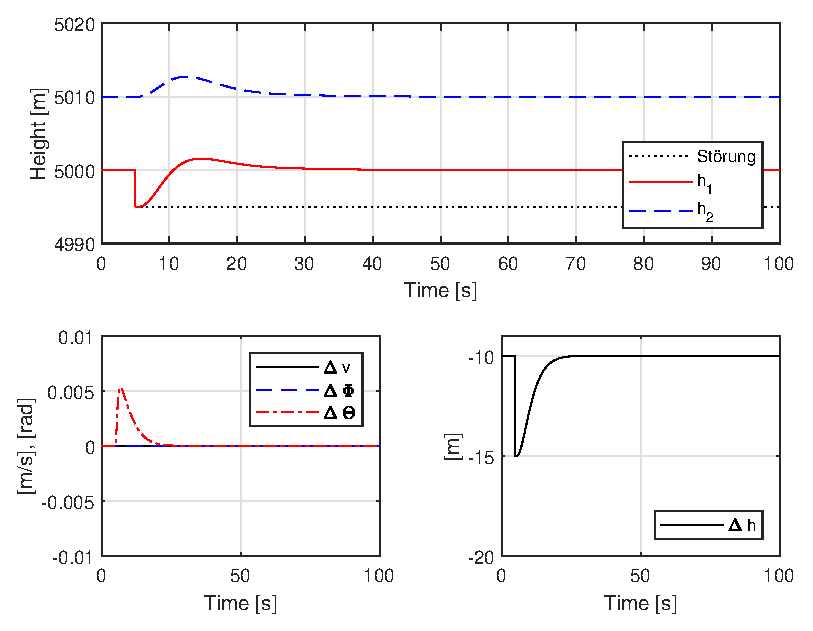
\includegraphics[width=\linewidth]{./Bilder/outputs_luftloch.eps}
 		\caption{Einfluss des Luftlochs auf die Höhe und die verkoppelten Ausgänge des nichtlinearen Modells}
 		\label{fig:outputs_luftloch}
 	\end{subfigure}
 	\hfill
 	\begin{subfigure}{.49\textwidth}
 		\centering
 		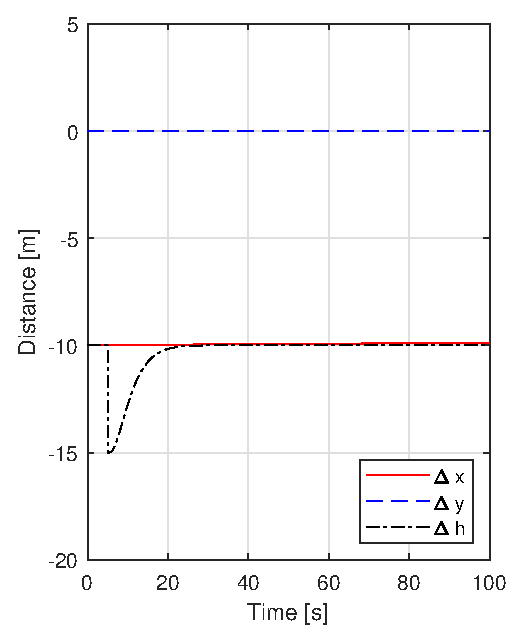
\includegraphics[width=0.65\linewidth]{./Bilder/distance_xyz_luftloch.eps}
 		\caption{Einfluss des Luftlochs auf die Positionsdifferenz der Flugzeuge beim nichtlinearen Modell}
 		\label{fig:distance_xyz_luftloch}
 	\end{subfigure}
 	\caption{Systemverhalten bei Störung durch ein Luftloch von \valunit{5}{m}}
 	\label{fig:luftloch}
 \end{figure}

\subsection{Störung durch Wind}
Störungen durch Windeinflüsse werden ebenfalls als sprungförmig modelliert. Dazu wird das in \Simulink\, implementierte Windmodell "Discrete Wind Gust Model \cite{windmodel}"\, verwendet, welches Windböen bezüglich der drei körperfesten Geschwindigkeitsachsen eines Flugzeugs erzeugt. Die Windböen nehmen dabei direkten Einfluss auf die Geschwindigkeit des Flugzeugs. Die Stärke der Windböen wird motiviert durch \cite{pollini} zu $\begin{bmatrix}
u_w, v_w, w_w
\end{bmatrix}^\transp = \begin{bmatrix}
0.5, 3.5, 0.5 
\end{bmatrix}^\transp$ \unit{m/s} gewählt - die Windböe wirkt also maßgeblich in Querrichtung der Flugzeuge. In diesem Fall wird angenommen, dass beiden Flugzeuge den Windböen gleichermaßen ausgesetzt sind. 
Die Windboe ist in Abbildung \ref{fig:windboe} gezeigt. Sie beginnt nach \valunit{10}{s}, ist über einen Zeitraum von \valunit{50}{s} konstant und klingt anschließend wieder ab.
 \begin{figure}[h] % figure störung windböe
	\centering
	\begin{subfigure}{.49\textwidth}
		\centering
		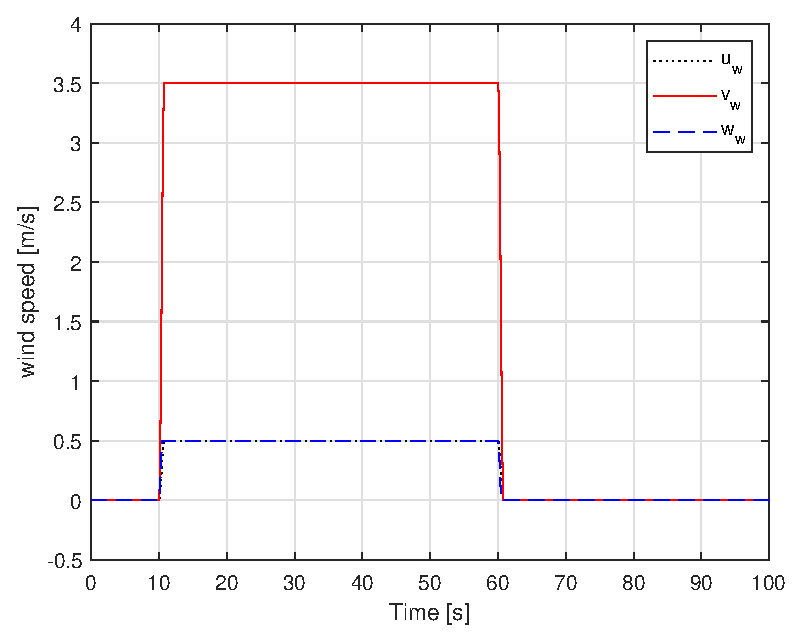
\includegraphics[width=\linewidth]{./Bilder/windboe.eps}
		\caption{Die drei Geschwindigkeitskomponenten der Windböe}
		\label{fig:windboe}
	\end{subfigure}
	\hfill
	\begin{subfigure}{.49\textwidth}
		\centering
		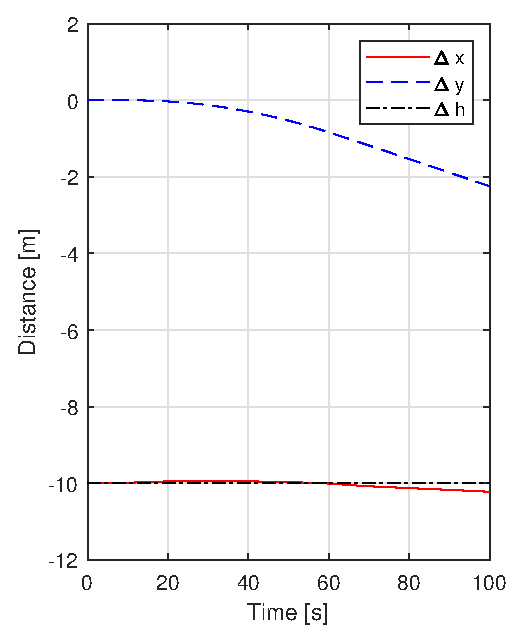
\includegraphics[width=0.65\linewidth]{./Bilder/distance_xyz_windboe.eps}
		\caption{Einfluss der Windböe auf die Positionsdifferenz der Flugzeuge beim nichtlinearen Modell}
		\label{fig:distance_xyz_windboe}
	\end{subfigure}
	\caption{Störung durch eine Windböe}
	\label{fig:pos_windboe}
\end{figure}

In Abbildung \ref{fig:outputs_windboe} ist das Systemverhalten unter Einfluss der Windstörung dargestellt. Abbildung \ref{fig:outputs_y1_windboe} zeigt den Einfluss auf die Höhen der Flugzeuge sowie den Einfluss auf die Ausgänge $v_1, \Phi_1$ und $\Theta_1$. Es ist deutlich erkennbar, dass die Windböe zu einem Auf- bzw. Abschwingen der einzelnen Größen führt. Die Flugzeuge schwingen in ihrer Höhe jeweils um \valunit{90}{cm}, wobei der Einfluss nach jeweils \valunit{20}{s} abgeklungen ist. Auch bei dieser Störung zeigt sich, dass Flugzeug 2 dem Verhalten von Flugzeug 1 im Sinne der Verkopplung folgt, obwohl für seine Ausgänge keine separate Unterlagerung entworfen wurde. Die Ausgänge $v_1, \Phi_1$ und $\Theta_1$ werden ebenfalls durch die Windböe beeinflusst und weichen von ihren Arbeitspunkten ab. Die Geschwindigkeitskomponente $v_1$ weicht um \valunit{0.18}{m/s} ab, wird jedoch nach \valunit{6}{s} zurück auf ihren Sollwert ausgeregelt. Die Abweichung bei $\Phi_1$ beträgt \valunit{0.025}{rad}, bei $\Theta_1$ \valunit{0.003}{rad}. Der Einfluss auf diese Größen ist damit äußerst gering. Es zeigt sich, dass die Windböe durch die Unterlagerung stationär genau ausgerelt wird. In Abbildung \ref{fig:outputs_ycoupl_windboe} ist der Einfluss auf die verkoppelten Ausgänge dargestellt. Auch hier ist gut zu erkennen, dass der Einfluss durch die Windböe marginal ist und die Verkopplung der einzelnen Größen, bis auf Abweichungen $<1\eexp{-03}$, erhalten bleibt.
\begin{figure}[H] % figure outputs windböe
	\centering
	\begin{subfigure}{0.49\textwidth}
		\centering
		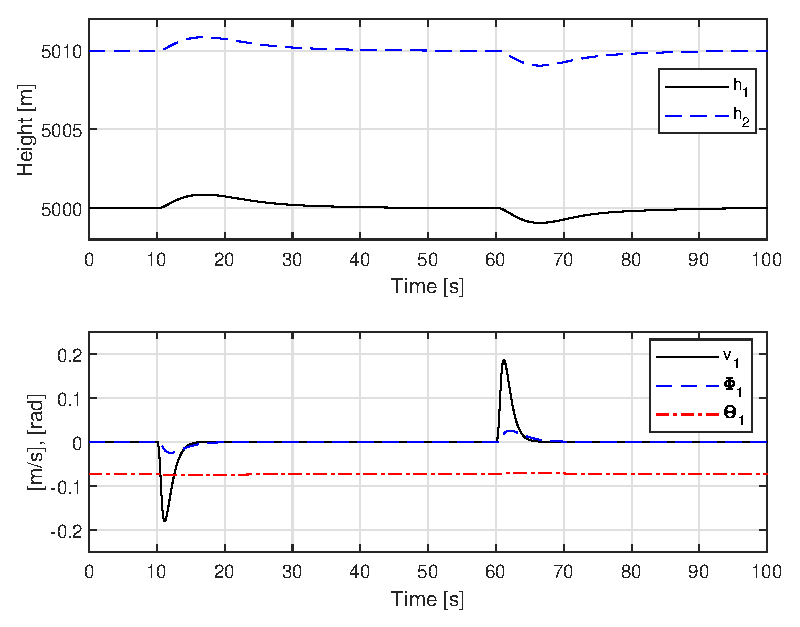
\includegraphics[width=\linewidth]{./Bilder/outputs_y1_windboe.eps}
		\caption{Einfluss der Windböe auf die Höhe der Flugzeuge 1 und 2 und die Ausgänge von Flugzeug 1 beim nichtlinearen Modell}
		\label{fig:outputs_y1_windboe}
	\end{subfigure}
	\hfill
	\begin{subfigure}{0.49\textwidth}
		\centering
		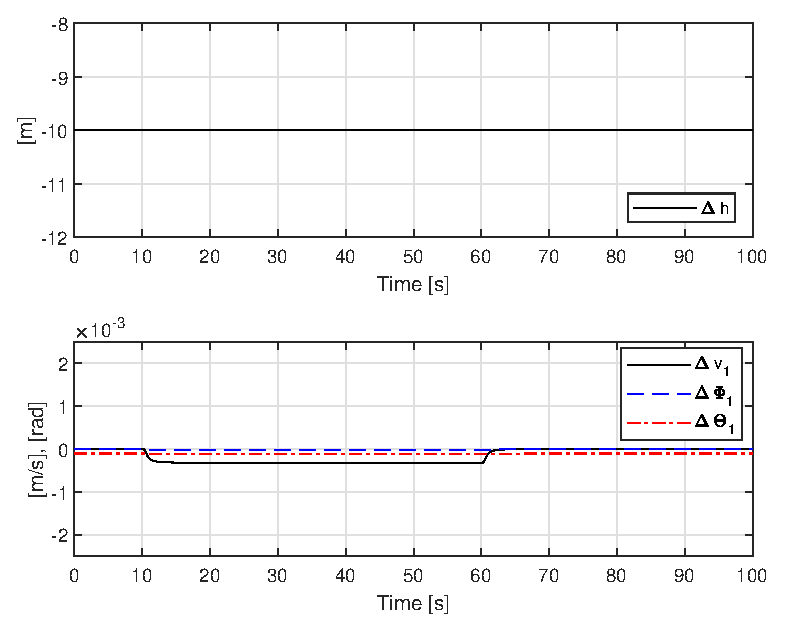
\includegraphics[width=\linewidth]{./Bilder/outputs_ycoupl_windboe.eps}
		\caption{Einfluss der Windböe auf die verkoppelten Ausgänge der Flugzeuge beim nichtlinearen Modell}
		\label{fig:outputs_ycoupl_windboe}
	\end{subfigure}
	\caption{Systemverhalten bei Störung durch eine Windböe}
	\label{fig:outputs_windboe}
\end{figure} 

Der Einfluss der Windböe auf die Positionsdifferenzen der Flugzeuge ist in Abbildung \ref{fig:distance_xyz_windboe} dargestellt. Trotz der Verkopplung der Ausgangsgrößen ist eine deutliche Abweichungen der Flugzeugpositionen zu erkennen. Sowohl in $x-$Richtung als auch in $y-$Richtung weichen die Positionen der Flugzeuge von einander ab. Während die Abweichung in $x-$Richtung relativ gering ist, beträgt die Abweichung in $y-$Richtung nach \valunit{100}{s} bereits über \valunit{2}{m}. Damit lässt sich schlussfolgern, dass die Windböe, welche auf beide Flugzeuge gleichermaßen einwirkt, zwar unter Beibehaltung der Verkopplung für die Ausgänge $v, \Phi, \Theta$ und $h$ stationär genau ausgeregelt wird. Die Verkopplung der Positionen ist allerdings bei Wirken der Störung nicht mehr gegeben, was daran liegt, dass die Positionen in der Regelschleife nicht enthalten sind.

\section{Probleme bei der Lösbarkeit des Optimierungsproblems mit \texttt{gammasyn}}
Wie bereits erläutert, wurde zur Regleroptimierung die \Matlab Toolbox \texttt{gammasyn} des IAT verwendet. Im Laufe dieses Projekts traten an mehreren Stellen immer wieder Fehler bei der Optimierung auf und führten zu unerwarteten Problemen. In diesem Abschnitt wird auf diese Fehler eingegangen. Zum einen soll dies der Transparenz der zum Reglerentwurf durchgeführten Schritte dienen. Zum anderen soll dies dazu dienen, Personen, die sich im Anschluss an dieses Projekt mit dem Thema beschäftigen, darauf aufmerksam zu machen, an welchen Stellen Probleme auftreten können und worin unter Umständen Verbesserungspotential für das Modell und die verwendeten Methoden besteht. Sofern nicht explizit anders erklärt, wurde für das Herbeiführen der hier beschriebenen Probleme nur das nominelle Modell verwendet.

\subsection{Entfernen kleiner Werte ($<\eexp{-09}$) aus den Matrizen}
Numerisch sehr kleine Werte, von denen man zunächst keine numerische Relevanz erwarten würde, \textbf{nicht} aus den Systemmatrizen \mat{A} und \mat{B} entfernt. Ein Entfernen dieser Werte führt in \texttt{gammasyn} bei ansonsten unveränderten Parametern zu einem Rangabfall in der Constraint Matrix und dadurch zu einem Fehler, was auf ein nicht lösbares Gleichungssystem hindeutet. 

In Kapitel \ref{cha:Regler} wurde ebenfalls erklärt, dass jene kleine Werte aus den Initialwerten $\mat{K}_\tn{init}$ und $\mat{F}_\tn{init}$ der Optimierung explizit entfernt wurden. Hier zeigte sich, dass gegenteiliges Vorgehen zwar zu einem erfolgreichen Entwurf führt, das Ergebnis jedoch stark von dem ursprünglichen Ergebnis abweicht. Es werden vollkommen andere Reglermatrizen $\mat{K}_\tn{koppel}$ und $\mat{F}_\tn{mod}$ erzielt, was zu anderen Pollagen führt. Das Systemverhalten dieser Regler führte auch bei der Führungsgröße $h_1$ zu enorm hohen Stellgrößen und damit zu instabilem Verhalten, weshalb diese Ergebnisse nicht weiter betrachtet wurden. 

Es lässt sich also insgesamt festhalten, dass je nach Startwert und Entfernen numerisch sehr kleiner Werte, mit dem in dieser Arbeit verwendeten Modell vollkommen verschiedene Ergebnisse, bis hin zu nicht lösbaren Optimierungsproblemen erzielt werden. 

\subsection{Variation des Arbeitspunktes}
Ähnlich zu der zuvor beschriebenen Abhängigkeit bezüglich der Startwerte, konnte festgestellt werden, dass auch eine Variation des Arbeitspunktes unter Umständen zu einem nicht lösbaren Gleichungssytem in der Optimierung führen kann. Wird beispielsweise die Geschwindigkeit der Flugzeuge im Arbeitspunkt von $u_{1\tn{AP}} = u_{2\tn{AP}} = \valunit{150}{m/s}$ auf $u_{1\tn{AP}} = u_{2\tn{AP}} = \valunit{130}{m/s}$ verringert, so lässt sich immer noch ein stabiler Arbeitspunkt für den Geradeausflug bestimmen. Allerdings schlägt die Optimierung auch hier wider Erwarten aufgrund eines nicht lösbaren Gleichungssystems fehl. Dies gilt sowohl für das ursprünglich verwendete Polgebiet, welches in Kapitel \ref{cha:Regler} erklärt wurde, als auch für Polgebiete, welche nur die Imaginärachse der komplexen s-Halbebene als Mindestanforderung besitzen oder Polgebiete, die sogar instabiles Verhalten zulassen.

\subsection{Parameterschwankung in der Masse bei Verwendung eines einzelnen Modells}
Ein weiterer Problemfall tritt auf, wenn anstelle des nominellen Modells eines der Modelle 2 (vor der Betankung) oder 3 (nach der Betankung) verwendet wird. Wenn man nun versucht einen Regler nur für Modell 2 unter Beibehaltung der Startwerte und des Polgebiets aus Kapitel \ref{cha:Regler} auszulegen, dann führt das gemäß der Erklärungen in Abschnitt \ref{sec:Parameterschwankungen} zu unterschiedlichen Arbeitspunkten für die beiden Flugzeuge. Wird nun die Treibstoffmasse über den Parameter $t\in[0,1]$ variiert, kann dies aufgrund von Rangfehlern zu einem nicht lösbaren Gleichungssystem bei der Optimierung führen. Nachfolgend werden dazu beispielhaft einige Werte für $t$ genannt, die zu lösbaren bzw. unlösbaren Gleichungssystemen führen.
\begin{table}[h]
\begin{center}
 \begin{tabular}{||c c c||} 
	\hline
	$t$ & lösbar & nicht lösbar \\ [0.5ex] 
	\hline
	0.1 & X & - \\
	0.5 & X & - \\
	0.8 & - & X \\
	0.9 & X & - \\
	1 & - & X \\
	1.1 & X & - \\
	1.3 & - & X \\
	1.4 & X & - \\
	\hline
\end{tabular}
\caption{\label{tab:parameterschwankung_t} Lösbarkeit des Gleichungssystems bei der Optimierung für Modell 2 in Abhängigkeit der Treibstoffmasse.}
\end{center}
\end{table} 
Tabelle \ref{tab:parameterschwankung_t} stellt dar, ob die Optimierung für Modell 2 bei entsprechender Wahl von $t$ für die Treibstoffmasse zu einem lösbaren oder nicht lösbaren Gleichungssystem innerhalb der Optimierung führt. Wie zu erkennen ist, gibt es keine eindeutige Abgrenzung, ab der der Massenunterschied der beiden Flugzeuge aufgrund des Treibstoffs zu groß wird. Viel mehr liegt hier die Vermutung nahe, dass die Lösbarkeit des Optimierungsproblems und damit auch die Tatsache, ob ein Verkopplungsregler für das System gefunden werden kann, stark von der Masse des Treibstoffs abhängt.

\subsection{Entfernen der Verkopplungsbedingung für $\Delta \Theta$}
Die Auswertung des linearen Modells hat bereits gezeigt, dass die Vorgabe von $\Theta_1$ mit dem Verkopplungsregler zu sehr hohen Stellgrößen und damit zu instabilem Verhalten führen kann, falls die Stellgrößen beschränkt werden. Dazu kommt die Vermutung, dass die Forderung zwei Flugzeuge, die unterschiedliche Massen und damit verschiedene Arbeitspunkte besitzen, sowohl in ihrer Höhe als auch in ihrem Nickwinkel miteinander zu verkoppeln, nur schwer umsetzbar ist. Die unterschiedlichen Massen führen dazu, dass das Systemverhalten der beiden Flugzeuge nicht mehr übereinstimmt. Eine Möglichkeit diese Problematik zu umgehen, ist der Ansatz die Verkopplungsbedingung für $\Delta \Theta$ zu entfernen und stattdessen $\Theta_2$ ebenfalls als Regelgröße einzuführen. Dieser Ansatz führt allerdings auch bereits bei der minimalen Forderung nach Stabilität zu einem Rangfehler in der Optimierung und damit zu einem nicht lösbaren Gleichungssystem.